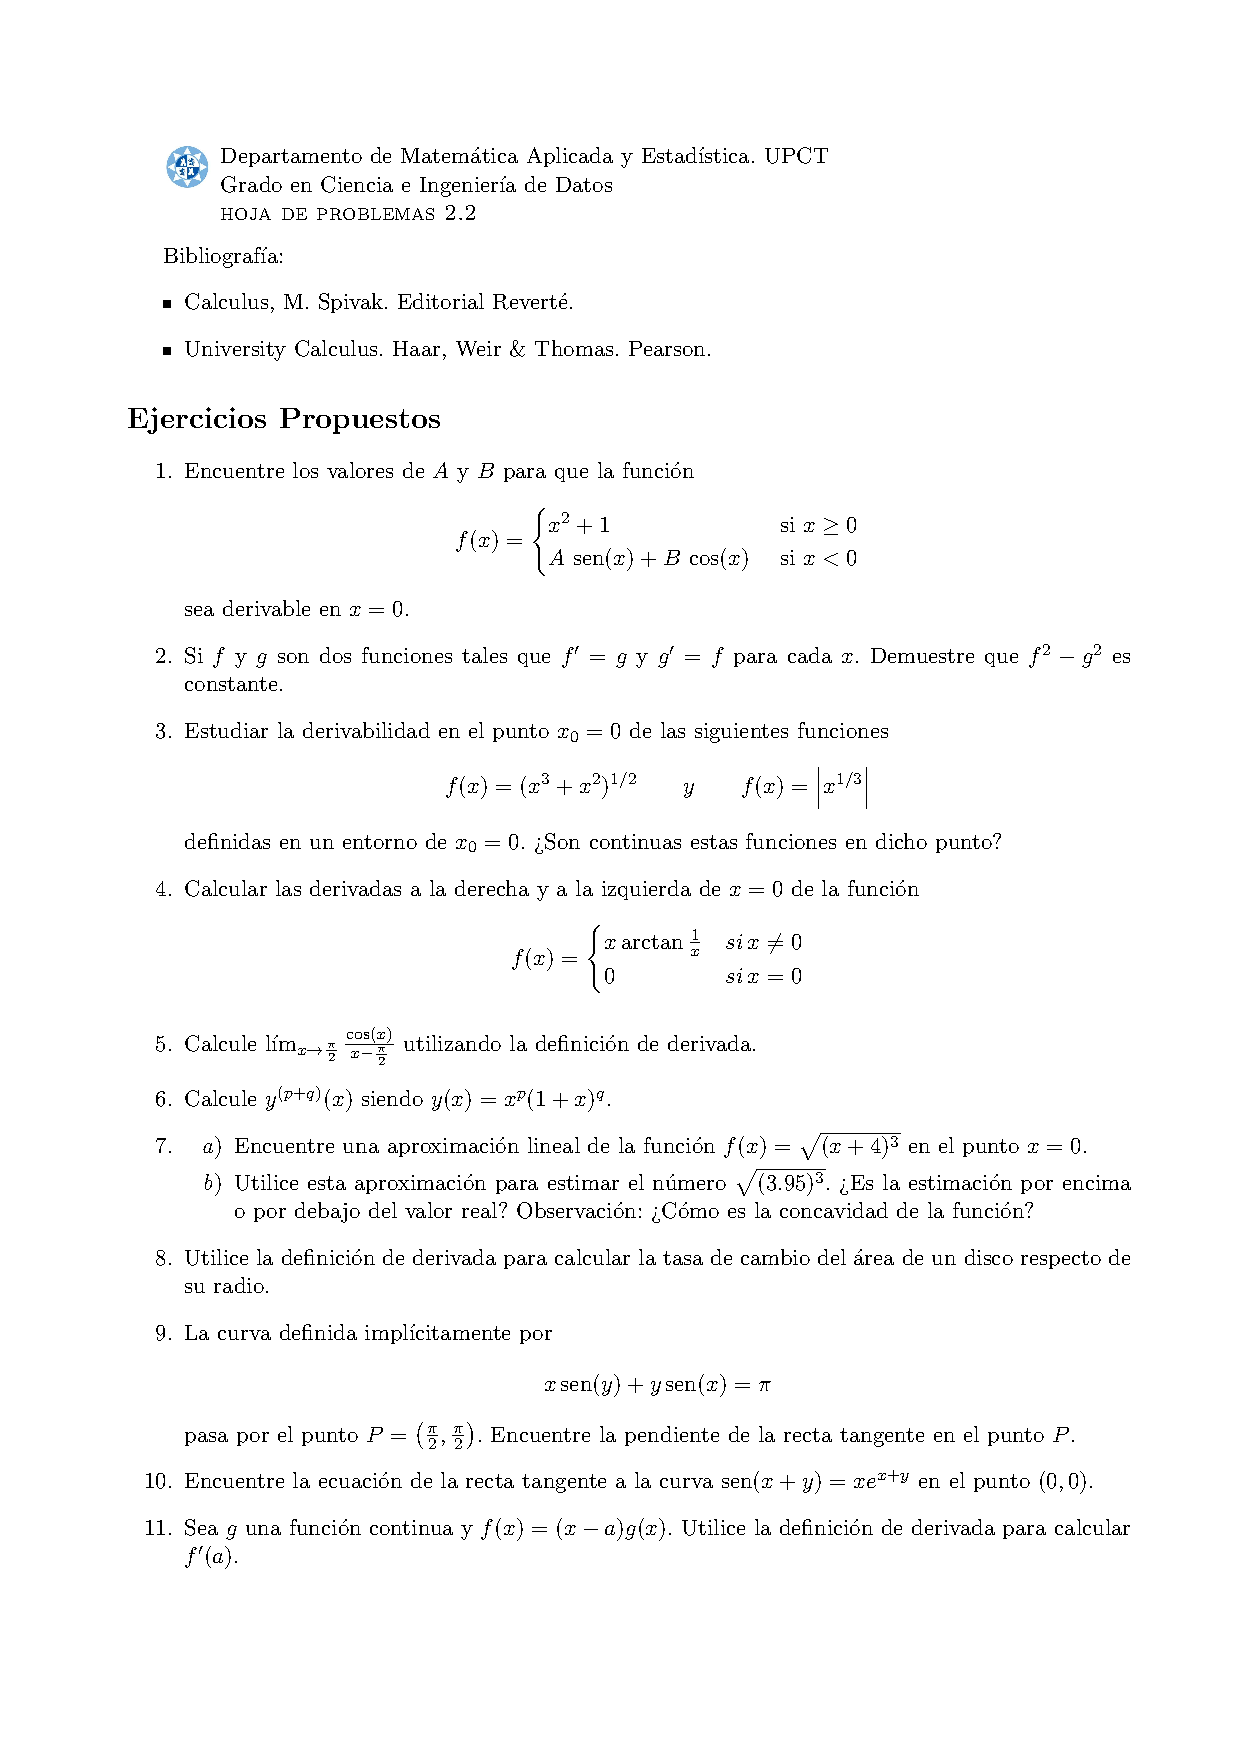
\includepdf[pages=-]{"Tema 2/Hoja 2.2/Hoja 2.2.pdf"}

\begin{enumerate}[label=\color{red}\textbf{\arabic*)}, leftmargin=*]
	\item \lb{Encuentre los valores de $A$ y $B$ para que la función \[ f(x)=\begin{cases}
			x^2+1 & \text{si }x\ge0\\
			A\sin(x)+B\cos(x) & \text{si }x<0
		\end{cases} \] sea derivable en $x=0$.}
	
	$\begin{array}{l}
		\begin{rcases}
		\lim_{x\to0^+}x^2+1=1=f(0)\\
		\lim_{x\to0^-}A\sin(x)+B\cos(x)=B=1
	\end{rcases}\\
	\lim_{x\to0}\dfrac{f(x)-f(0)}{x}\left\langle\begin{array}{l}
	\lim_{x\to0^+}\dfrac{x^2+1-1}{x}=\lim_{x\to0^+}x=0\\
		\lim_{x\to0^-}\dfrac{A\sin(x)-\cos(x)-1}{x}=\lim_{x\to0}\dfrac{A\sin(x)}{x}+\lim_{x\to0}\dfrac{\cos(x)-1}{x}=A+0=A\longrightarrow A=0
	\end{array}\right.
	\end{array}$
	\item \lb{Si $f$ y $g$ son dos funciones tales que $f'=g$ y $g'=f$ para cada $x$. Demuestre que $f^2-g^2$ es constante.}
	
	$(f^2-g^2)'=2f\cdot f'-2 g\cdot g'=2fg-2gf=0$
	\item \lb{Estudiar la derivabilidad en el punto $x_0=0$ de las siguientes funciones \[ f(x)=(x^3+x^2)^{\frac{1}{2}}\qquad\mathrm{y}\qquad f(x)=\left|x^{\frac{1}{3}}\right| \] definidas en un entorno de $x_0=0$. ¿Son continuas estas funciones en dicho punto?}
	
	$\begin{array}{l}
		x_0=0\qquad x^3+x^2\ge0\qquad x^2(x+1)\ge0\qquad x\ge -1\\
		f(x)=\sqrt{x^3+x^2}=(x^3+x^2)\\
		f'(x)=\dfrac{1}{2\sqrt{x^3+x^2}}\cdot(3x^2+2x)=\dfrac{x(3x+2)}{2|x|\cdot\sqrt{x+1}}\\
		f(0)=0\\
		\lim_{x\to0^+}\dfrac{f(x)-f(0)}{x}=\lim_{x\to0}\dfrac{\sqrt{x^3+x^2}}{x}=\lim_{x\to0^+}\dfrac{|x|\sqrt{x+1}}{x}=1\\
		\lim_{x\to0^-}\dfrac{f(x)-f(0)}{x}=\lim_{x\to0^-}\dfrac{|x|\sqrt{x+1}}{x}=\lim_{x\to0^-}\dfrac{-\cancel{x}\sqrt{x+1}}{\cancel{x}}=-1
	\end{array}$
	\item \lb{Calcular las derivadas a la derecha y a la izquierda de $x=0$ de la función \[ f(x)=\begin{cases}
			x\arctan\dfrac{1}{x} & \text{si }x\neq0\\
			0 & \text{si }x=0
		\end{cases} \] definidas en un entorno de $x_0=0$. ¿Son continuas estas funciones en dicho punto? }
	
	$\begin{array}{l}
		f(x)=\begin{cases}
		\arctan & x\neq0\\
		0 & x=0
	\end{cases}\\
	\lim_{x\to0^+}\arctan\left(\dfrac{1}{x}\right)=\dfrac{\pi}{2}\\
	\lim_{x\to0^-}\arctan\left(\dfrac{1}{x}\right)=-\dfrac{\pi}{2}\\
	\lim_{x\to0}x\cdot\arctan\left(\dfrac{1}{x}\right)\left\langle\begin{array}{l}
		\lim_{x\to0^+}x\cdot\arctan\left(\dfrac{1}{x}\right)=0\cdot\dfrac{\pi}{2}=0\\
		0\cdot\left(-\dfrac{\pi}{2}\right)=0
	\end{array}\right.
	\end{array}$
	
\begin{center}
	\begin{tikzpicture}
		\begin{axis}[
			axis lines=center,
			]
			\addplot[lightblue, domain=-pi/2:pi/2,samples=200] {tan(deg(x))};
		\end{axis}
	\end{tikzpicture}
	\hspace{1cm}
	\begin{tikzpicture}
		\begin{axis}[
			axis lines=center,
			]
			\addplot[lightblue,domain=-3:3,samples=200] {atan(x)};
		\end{axis}
	\end{tikzpicture}
\end{center}
	\item \lb{Calcule $\lim_{x\to\frac{\pi}{2}}\dfrac{\cos(x)}{x-\frac{\pi}{2}}$ utilizando la definición de derivada.}
	
	$\begin{aligned}
		\lim_{x\to\frac{\pi}{2}}\dfrac{\cos(x)}{x-\frac{\pi}{2}}=\lim_{x\to\frac{\pi}{2}}\dfrac{\cos(x)-\cos\left(\frac{\pi}{2}\right)}{x-\frac{\pi}{2}}&=\left(\cos(x)\right)'_{x=\frac{\pi}{2}}\\
		&=\left(-\sin(x)\right)_{x=\frac{\pi}{2}}=-1
	\end{aligned}$
	\item \lb{Calcule $y^{(p+q)}(x)$ siendo $y(x)=x^p(1+x)^q$.}
	
	Supongamos $p\ge q$\\
	$\begin{array}{l|l}
		g(x)=x^+ & h(x)=(1+x)^q\\
		g'(x)=p\cdot x^{p-1} & h'(x)=q\cdot(1+x)^{q-1}\\
		g''(x)=p\cdot(p-1)\cdot p^{p-2} & \vdots\\
		\vdots & h^{q)}(x)=q!\\
		g^{p)}(x)=p! & h^{n)}(x)=0\quad\text{para }n\ge q\\
		g^{n)}(x)=0\quad\text{para }n\ge p &
	\end{array}$
	
	$y^{(p-q)}(x)=\sum_{n=0}^{p+q}\binom{p+q}{n}\cdot g^{n)}(x)\cdot h^{p+q\cdot n)}(x)$
	\item \begin{enumerate}[label=\color{red}\alph*)]
		\item \lb{Encuentre una aproximación lineal de la función $f(x)=\sqrt{(x+4)^3}$ en el punto $x=0$.}
		
		$\begin{array}{l}
			f(x)=\sqrt{(x+4)}^3\qquad x=0\qquad f(0)=\sqrt{4^3}=8\\
			P(x)=f(0)+\dfrac{f'(0)}{1!}\cdot(x-0)=8+3x\\
			f'(x)=\dfrac{3}{2}(x+4)^{\frac{1}{2}}\\
			f'(0)=3
		\end{array}$\qquad\begin{tikzpicture}[baseline=(current bounding box.center)]
		\begin{axis}[axis lines=center]
			\addplot[lightblue, samples=200, line width=1.5pt] {sqrt((x+4)^3)};
			\addplot[blue,samples=200, line width=1.5pt] {8+3*x};
		\end{axis}
		\end{tikzpicture}
		\item \lb{Utilice esta aproximación para estimar el número $\sqrt{(3.95)^3}$. ¿Es la aproximación por encima o por debajo del valor real? Observación: ¿Cómo es la concavidad de la función?}
	\end{enumerate}
	\item \lb{Utilice la definición de derivada para calcular la tasa de cambio del área de un disco respecto de su radio.}
	\item \lb{La curva definida implícitamente por \[ x\sin(y)+y\sin(x)=\pi \] pasa por el punto $P=\left(\dfrac{\pi}{2},\dfrac{\pi}{2}\right)$. Encuentre la pendiente de la recta tangente en el punto $P$.}
	\item \lb{Encuentre la ecuación de la recta tangente a la curva $\sin(x+y)=xe^{x+y}$ en el punto $(0,0)$.}
	
	$\underset{0}{\sin(0+0)}=\underset{0}{0\cdot e^{0+0}}$
	
	Derivamos respecto de $x$
	
	$\begin{aligned}
		\cos(x+y)\cdot(1+y')&=1\cdot e^{x+y}+x\cdot e^{x+y}\cdot(1+y')\\
		1+y'(0)&=1\longrightarrow\bboxed{y'(0)=0}
	\end{aligned}$
	\item \lb{Sea $g$ una función continua y $f(x)=(x-a)g(x)$. Utilice la definición de derivada para calcular $f'(a)$.}
	\item \lb{Calcula la función derivada de las siguientes funciones:}
	\begin{enumerate}[label=\color{red}\alph*)]
		\item $\db{f(x)=\sqrt{x+\sqrt{x+\sqrt{x}}}, x>0}$
		\item $\db{f(x)=\left(\dfrac{1-x}{1+x}\right)^{2\log(1+x)}, x>-1}$
		\item $\db{f(x)=x^{\arcsin(x)}, x>0}$
	\end{enumerate}
      \item 
      \item 
      \item \lb{}
      
      \begin{tikzpicture}
            \draw (-1,0) -- (3,0);
            \draw (0,-1) -- (0,5);
            \draw[lightblue] (0,0) rectangle (2,4);
            \node[lightblue, above] at (1,4) {$x$};
            \node[lightblue, below] at (1,0) {400 metros};
            \node[lightblue, right] at (2,2) {$y$};
            \node[lightblue, left] at (0,2) {100 metros};
      \end{tikzpicture}
      \item 
      \item \lb{}
      $A(y):[0,100]\longrightarrow\R^+$
      
      \begin{tikzpicture}
            \draw (-1,0) -- (6,0) node[above] {120 millas/h};
            \draw (0,-1) -- (0,6) node[midway,left] {3 millas};
            \draw[lightblue] (0, 6) -- (5,0);
            \draw[blue] (1,6) -- (4,0) |- (1,6) node[midway, below] {$4$};
            \draw[lightblue,dashed] (0,6) -- (1,6) ;
      \end{tikzpicture}
      
      $\begin{array}{l}
            4-120t-xt\\
            d(t)=\sqrt{(4-120t-xt)^2+9}\\
            d'(t)_{|t=0}=-160 \text{ millas/h}
      \end{array}\longrightarrow x=80$
\end{enumerate}